% Quadratic Penalty Figure: O/R-Regret Relationship
% This figure demonstrates the quadratic relationship between O/R Index and regret,
% showing that halving O/R reduces regret by approximately 75% (not 50%).

\begin{figure}[t]
\centering
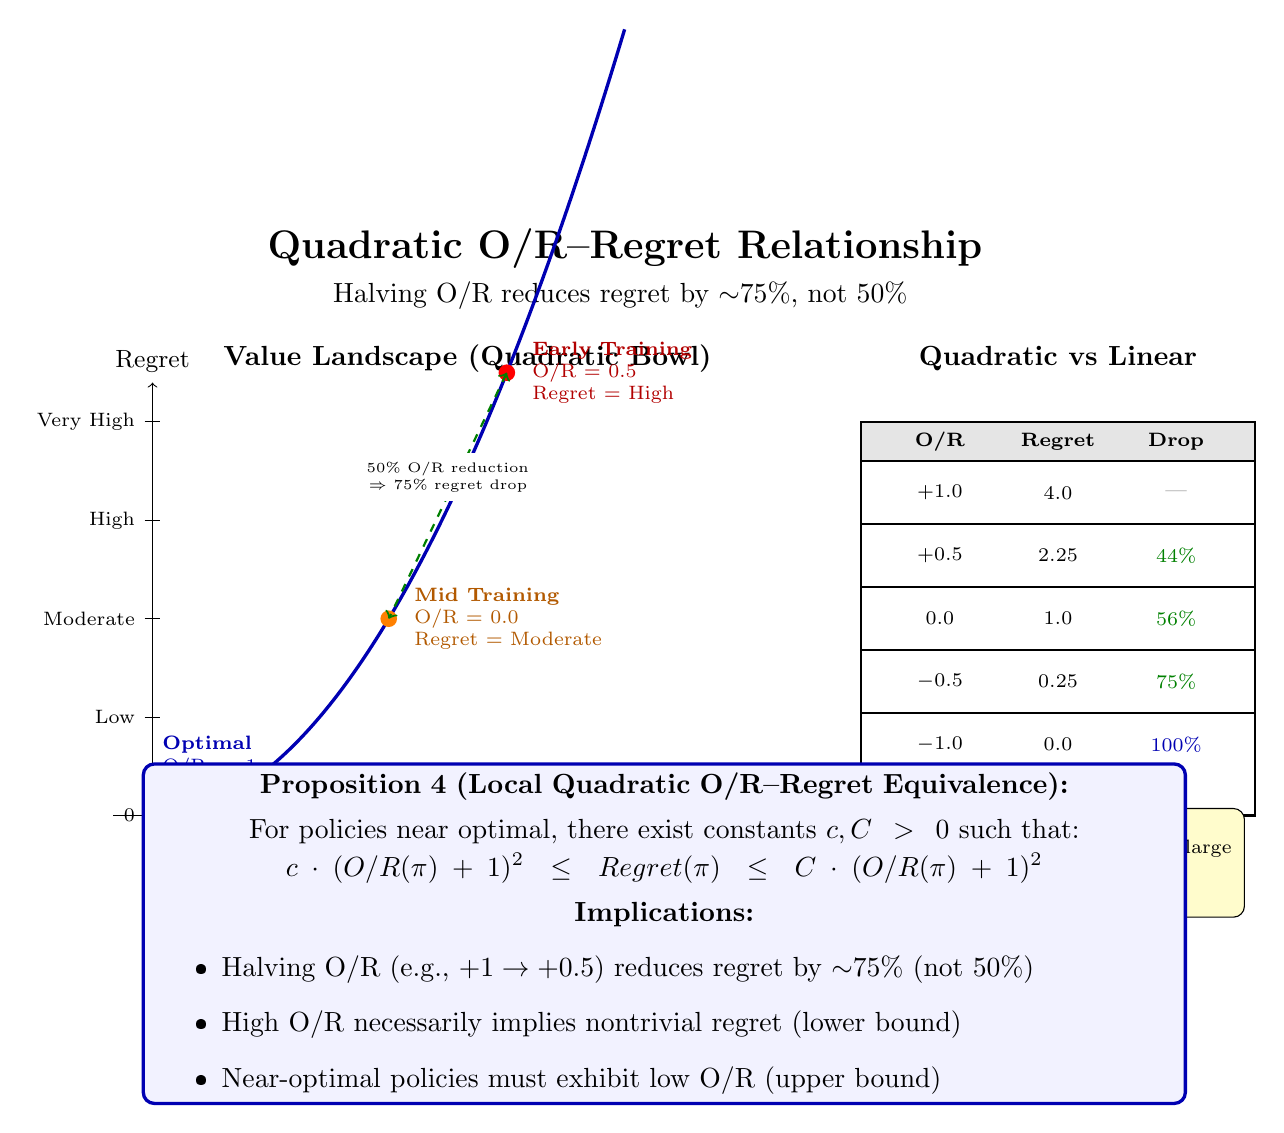
\begin{tikzpicture}[scale=1.0]

% Title
\node[font=\Large\bfseries] at (6, 7.2) {Quadratic O/R--Regret Relationship};
\node[font=\normalsize, align=center] at (6, 6.6) {
    Halving O/R reduces regret by $\sim$75\%, not 50\%
};

% LEFT PANEL: Quadratic Bowl
\begin{scope}[shift={(0,0)}]
    % Title
    \node[font=\bfseries, align=center] at (4, 5.8) {Value Landscape (Quadratic Bowl)};

    % Draw axes
    \draw[->] (-0.5, 0) -- (8, 0) node[right, font=\small] {O/R Index};
    \draw[->] (0, -0.5) -- (0, 5.5) node[above, font=\small] {Regret};

    % Draw quadratic curve: Regret = c*(O/R + 1)^2
    % O/R ranges from -1 (optimal) to +1 (worst)
    % Parametric: x = O/R, y = (O/R + 1)^2
    \draw[very thick, blue!70!black, domain=-1:1, samples=100, smooth]
        plot ({(\x+1)*3}, {(\x+1)*(\x+1)*2.5});

    % Axis ticks and labels
    \foreach \x/\label in {0/-1, 1.5/-0.5, 3/0, 4.5/0.5, 6/+1} {
        \draw (\x, -0.1) -- (\x, 0.1);
        \node[below, font=\scriptsize] at (\x, -0.1) {\label};
    }
    \foreach \y/\label in {0/0, 1.25/Low, 2.5/Moderate, 3.75/High, 5/Very High} {
        \draw (-0.1, \y) -- (0.1, \y);
        \node[left, font=\scriptsize] at (-0.1, \y) {\label};
    }

    % Mark key training phases
    % Early training: O/R ≈ 0.5
    \fill[red] (4.5, 5.625) circle (3pt);
    \node[right, font=\scriptsize, align=left, text=red!70!black] at (4.7, 5.625) {
        \textbf{Early Training}\\
        O/R = 0.5\\
        Regret = High
    };

    % Mid training: O/R ≈ 0.0
    \fill[orange] (3, 2.5) circle (3pt);
    \node[right, font=\scriptsize, align=left, text=orange!70!black] at (3.2, 2.5) {
        \textbf{Mid Training}\\
        O/R = 0.0\\
        Regret = Moderate
    };

    % Late training: O/R ≈ -0.7
    \fill[green!50!black] (0.9, 0.225) circle (3pt);
    \node[right, font=\scriptsize, align=left, text=green!50!black] at (1.1, 0.225) {
        \textbf{Late Training}\\
        O/R = -0.7\\
        Regret = Low
    };

    % Optimal policy at O/R = -1
    \fill[blue!70!black] (0, 0) circle (3pt);
    \node[above right, font=\scriptsize, align=left, text=blue!70!black] at (0, 0.1) {
        \textbf{Optimal}\\
        O/R = -1\\
        Regret = 0
    };

    % Annotation: Quadratic relationship
    \draw[<->, thick, dashed, green!50!black] (4.5, 5.625) -- (3, 2.5);
    \node[font=\tiny, align=center, fill=white] at (3.75, 4.3) {
        50\% O/R reduction\\
        $\Rightarrow$ 75\% regret drop
    };
\end{scope}

% RIGHT PANEL: Comparison Table
\begin{scope}[shift={(9,0)}]
    % Title
    \node[font=\bfseries, align=center] at (2.5, 5.8) {Quadratic vs Linear};

    % Draw table
    \draw[thick] (0, 5) rectangle (5, 0);

    % Header
    \draw[thick, fill=gray!20] (0, 5) rectangle (5, 4.5);
    \node[font=\scriptsize\bfseries] at (1, 4.75) {O/R};
    \node[font=\scriptsize\bfseries] at (2.5, 4.75) {Regret};
    \node[font=\scriptsize\bfseries] at (4, 4.75) {Drop};

    % Row 1: O/R = 1.0
    \draw[thick] (0, 4.5) -- (5, 4.5);
    \node[font=\scriptsize] at (1, 4.1) {$+1.0$};
    \node[font=\scriptsize] at (2.5, 4.1) {$4.0$};
    \node[font=\scriptsize, text=gray] at (4, 4.1) {---};

    % Row 2: O/R = 0.5
    \draw[thick] (0, 3.7) -- (5, 3.7);
    \node[font=\scriptsize] at (1, 3.3) {$+0.5$};
    \node[font=\scriptsize] at (2.5, 3.3) {$2.25$};
    \node[font=\scriptsize, text=green!50!black] at (4, 3.3) {44\%};

    % Row 3: O/R = 0.0
    \draw[thick] (0, 2.9) -- (5, 2.9);
    \node[font=\scriptsize] at (1, 2.5) {$0.0$};
    \node[font=\scriptsize] at (2.5, 2.5) {$1.0$};
    \node[font=\scriptsize, text=green!50!black] at (4, 2.5) {56\%};

    % Row 4: O/R = -0.5
    \draw[thick] (0, 2.1) -- (5, 2.1);
    \node[font=\scriptsize] at (1, 1.7) {$-0.5$};
    \node[font=\scriptsize] at (2.5, 1.7) {$0.25$};
    \node[font=\scriptsize, text=green!50!black] at (4, 1.7) {75\%};

    % Row 5: O/R = -1.0 (optimal)
    \draw[thick] (0, 1.3) -- (5, 1.3);
    \node[font=\scriptsize] at (1, 0.9) {$-1.0$};
    \node[font=\scriptsize] at (2.5, 0.9) {$0.0$};
    \node[font=\scriptsize, text=blue!70!black] at (4, 0.9) {100\%};

    % Key insight annotation
    \node[font=\scriptsize, align=left, text width=4.5cm, draw, rounded corners, fill=yellow!20] at (2.5, -0.6) {
        \textbf{Key:} Quadratic scaling means small O/R improvements yield large regret reductions.\\[2pt]
        $\text{Regret} \propto (\text{O/R} + 1)^2$
    };
\end{scope}

% BOTTOM: Mathematical relationship box
\node[font=\normalsize, align=center, text width=13cm, draw=blue!70!black, very thick, fill=blue!5, rounded corners] at (6.5, -1.5) {
    \textbf{Proposition 4 (Local Quadratic O/R--Regret Equivalence):}\\[4pt]
    For policies near optimal, there exist constants $c, C > 0$ such that:\\[2pt]
    $\displaystyle c \cdot (\text{O/R}(\pi) + 1)^2 \le \text{Regret}(\pi) \le C \cdot (\text{O/R}(\pi) + 1)^2$\\[4pt]
    \textbf{Implications:}
    \begin{itemize}
        \item Halving O/R (e.g., $+1 \to +0.5$) reduces regret by $\sim$75\% (not 50\%)
        \item High O/R necessarily implies nontrivial regret (lower bound)
        \item Near-optimal policies must exhibit low O/R (upper bound)
    \end{itemize}
};

\end{tikzpicture}

\caption{\textbf{Quadratic Relationship between O/R Index and Regret.}
\textbf{Left:} Value landscape showing the ``quadratic bowl'' structure. The optimal policy ($\text{O/R} = -1$) sits at the bottom. As O/R increases (more behavioral inconsistency), regret grows quadratically, not linearly. Training progresses from high O/R (early, red) through moderate (mid, orange) to low (late, green).
\textbf{Right:} Numerical comparison table demonstrating the quadratic scaling. Moving from O/R=$+0.5$ to O/R=$0.0$ (50\% reduction in O/R) yields a 56\% regret reduction; moving from O/R=$0.0$ to O/R=$-0.5$ yields an additional 75\% reduction. This quadratic relationship (Proposition 4) connects variance-based metrics to policy optimization theory, providing theoretical justification for using O/R as a coordination diagnostic.
The relationship $\text{Regret} \propto (\text{O/R} + 1)^2$ explains why small improvements in O/R during late-stage training can yield substantial performance gains.}
\label{fig:quadratic_or_regret}
\end{figure}
